\subsection{Constraints from LEP and electroweak precision data}

Very strong constraints on the i2HDM arise from precision data and searches from LEP experiments. First of all,
the model should respect the  precise measurements of the W and Z widths
which lead to the following lower limit on the odd scalar masses:
\begin{eqnarray}
\label{eq:constr-widths}
&& M_{h_1} + M_{h^{+}} > M_{W^{+}} \quad , \quad M_{h_2} + M_{h^{+}} > M_{W^{+}} \nonumber\\
&& M_{h_1} + M_{h_2} > M_{Z} \quad , \quad 2M_{h^{+}} > M_{Z}
\end{eqnarray}
to make sure that $\Gamma({W^{+} \rightarrow h_1 h^{+},h_2h^{+}})$ and $\Gamma({Z \rightarrow h_1h_2,h^+h^-})$ decay channels are kinematically 
forbidden.

While studying the phenomenology of the i2HDM, we should also make sure that 
Electroweak Precision Test (EWPT) data is respected.
As we know, EWPT can be  expressed in terms of three measurable quantities, called S, T, and U, that parameterise contributions
from beyond standard model physics  to electroweak radiative corrections~\cite{PhysRevD.46.381}.
The contribution to the S and T parameters~\cite{Barbieri:2006dq} can be written as
\begin{equation}
S = 
\frac{1}{72\pi}\frac{1}{(x_2^2-x_1^2)^3}
\left[ 
x_2^6 f_a(x_2) -x_1^6 f_a(x_1)
+ 9 x_2^2 x_1^2( x_2^2 f_b(x_2) - x_1^2 f_b(x_1)
\right]
\end{equation}
where $x_1=M_{h_1}/M_{h^+}, x_2=M_{h_2}/M_{h^+}$, $f_a(x) = -5+12\log(x), f_b(x)=3-4\log(x)$
and
%
\begin{equation}
T = \frac{1}{32\pi^2\alpha v^2}\left[f_c(M_{h^{+}}^2,M_{h_2}^2) + f_c(M_{h^{+}}^2,M_{h_1}^2) - f_c(M_{h_2}^2,M_{h_1}^2)\right]
\end{equation}
where the function $f_c(x,y)$ is defined by
\begin{equation*}
f_c(x,y) = 
\begin{cases}
\frac{x+y}{2}-\frac{xy}{x-y}\log{\left(\frac{x}{y}\right)}, & x\neq y\\
0, & x = y
\end{cases}
\end{equation*}
We have written the contributions to $S$ and $T$ in a form which demonstrates explicitly their symmetry
with respect to swapping $h_1 \leftrightarrow h_2$, pointing again to the fact that one can not distinguish their CP properties.
With $U$ fixed to be zero, the central values of $S$ and $T$, assuming a SM Higgs boson mass of $m_h$ = 125 GeV, are given by~\cite{Baak:2014ora}:
\begin{equation}
S = 0.06 \pm 0.09 ,\qquad T = 0.1 \pm 0.07
\label{eq:ewpt}
\end{equation}
with correlation coefficient +0.91.
The effect of the constraints on $S$ and $T$ is presented in  Fig.\ref{fig:s-t-u}, where panels a) and b)  present the 
colour map of the $S$ and  $T$ parameters respectively 
in the $(M_{h^+},M_{h_2})$ plane.
One can see that the $T$ variable is more  sensitive than $S$
to this mass split, thus only modest splits
are allowed by EWPT data.
Finally, Fig.\ref{fig:s-t-u} c) presents  the colour map
of the $M_{h^+}-M_{h_2}$  split in the ($S,T$) plane together with the
65\% and 95\% exclusion contours, based on a $\chi^2$ with  two degrees of freedom.
  One can see that
EWPT data prefer a modest positive $M_{h^+}-M_{h_2}$ mass split 
 below  about $100$ GeV, which is mainly defined by the $T$ parameter, while the role and the respective range of variation of $S$ is milder. One should stress that 
 it is crucial to take into account the correlation between
$S$ and $T$ and  combine limits from these two  parameters. This combination gives a much stronger limit on the parameter 
space, in particular on the $M_{h^+}-M_{h_2}$ mass split, while a much larger splitting would
naively be allowed by looking at the $S$ and $T$ values separately. This can be
seen from  Fig.\ref{fig:s-t-u}(a) and Fig.\ref{fig:s-t-u}(b) respectively.
  


\begin{figure}[htb]
\centering
\hspace*{-0.3cm}\subfigure[]{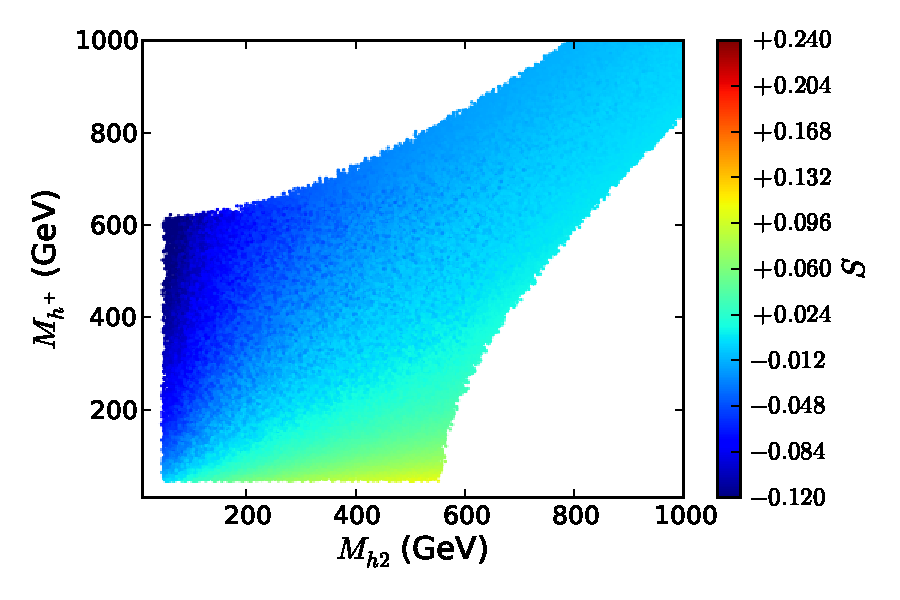
\includegraphics[width=0.55\textwidth]{Figures/Mh2_Mhp_S_cut123.pdf}}%
\hspace*{-0.3cm}\subfigure[]{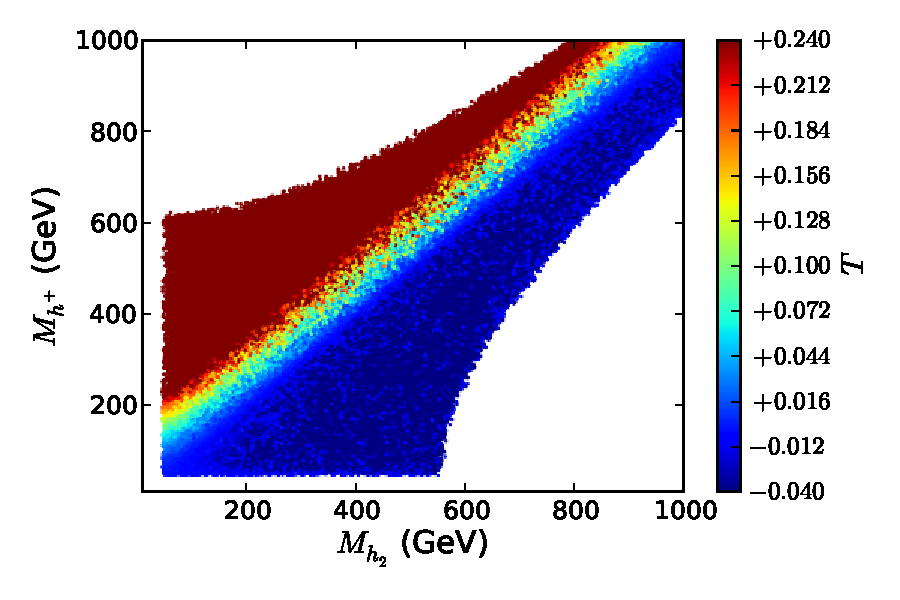
\includegraphics[width=0.55\textwidth]{Figures/Mh2_Mhp_T_cut123.pdf}}\\
\subfigure[]{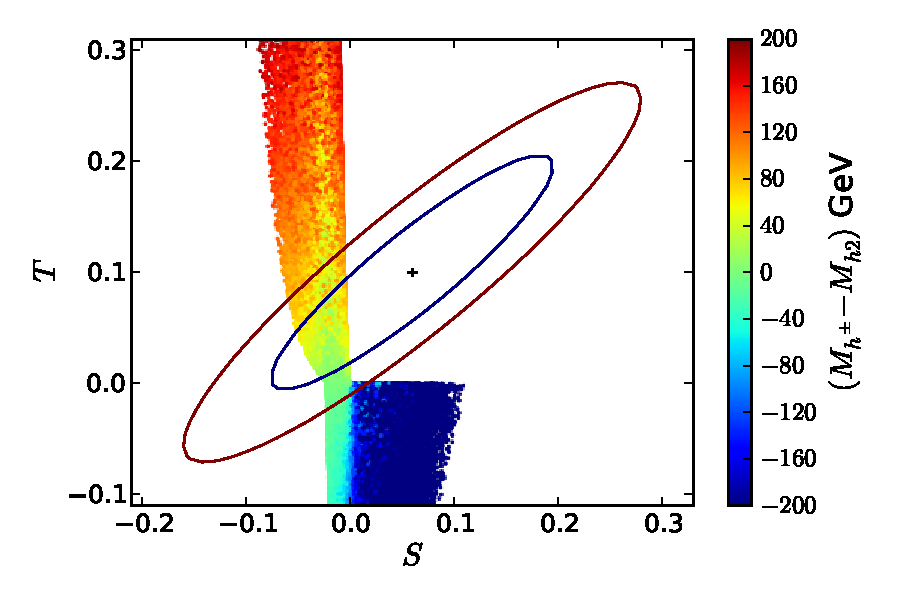
\includegraphics[width=0.55\textwidth]{Figures/S_T_Mhc-Mh2_cut123.pdf}}
\caption{
Effect of the  $S$ and $T$ constraints on the $M_{h^+}-M_{h_2}$ mass difference:
(a) and (b) show the 
colour map of the $S$ and  $T$ parameters respectively 
in the $(M_{h^+},M_{h_2})$ plane; (c) shows  the colour map
of the $M_{h^+}-M_{h_2}$ split in the ($S,T$) plane together with the
65\% and 95\% exclusion contours
based on the $\chi^2$ ($S,T$) characterisation for two degrees of freedom.} \label{fig:s-t-u}
\end{figure}


We also excluded the region defined by the intersection of the conditions below:
\begin{equation}
M_{h_1}<80\mbox{ GeV} \ , \ M_{h_2}<100\mbox{ GeV} \ ,  \ M_{h_2}-M_{h_1}>8 \mbox{ GeV}\,.
\label{eq:dmh12}
\end{equation}
This region is excluded by the LEP data since it would lead to a visible
di-jet or di-lepton signal as demonstrated in~\cite{Lundstrom:2008ai}
where a reinterpretation in the i2HDM of a LEP--II limit of the second neutralino production in the MSSM was presented.
A more detailed analysis of this specific region of the parameter space ---
low $M_{h_1}$ and $M_{h_2}$ with large enough mass gap --- was studied recently~\cite{Belanger:2015kga}.
One should also mention that  $e^+e^-\to h^+h^-$ production at LEP2
sets
\begin{equation}
M_{h^+}>70\mbox{ GeV}
\label{eq:mhcp-lep2}
\end{equation}
as found in~\cite{Pierce:2007ut} as a result of the re-interpretation of LEP--II limits on charginos.


